\documentclass[border=3pt]{standalone}
% Preâmbulo compartilhado pelos diagramas TikZ da aula
\usepackage[T1]{fontenc}
\usepackage[utf8]{inputenc}
\usepackage{lmodern}
\usepackage{amsmath}
\usepackage{xcolor}
\usepackage{tikz}
\usetikzlibrary{arrows.meta,angles,quotes,decorations.pathmorphing,calc,
                positioning,shapes.geometric,backgrounds,fit}

% Paleta (mesma dos SVGs originais)
\definecolor{dblue}{HTML}{2A5B8C}
\definecolor{dorange}{HTML}{B3541E}
\definecolor{dgreen}{HTML}{4A7C59}
\definecolor{dred}{HTML}{9C4B4B}
\definecolor{dcream}{HTML}{F4F1EA}
\definecolor{dshade}{HTML}{DDD7C9}

% Estilos comuns (prefixo d... para não colidir com chaves internas do pgf)
\tikzset{
  >={Stealth[length=2mm]},
  dguide/.style={gray!55, dashed, line width=0.4pt},
  daxis/.style={gray!60, line width=0.7pt, ->},
  dbody/.style={fill=black!3, draw=black!80, line width=1pt},
  dacc/.style={draw=dblue, line width=1pt},
  dlbl/.style={black!55, font=\small},
  dsub/.style={black!45, font=\footnotesize},
  dstate/.style={circle, draw=black!80, fill=dcream, line width=1pt,
                 minimum size=17mm, font=\large, inner sep=1pt},
  dobs/.style={circle, draw=black!80, fill=dshade, line width=1pt,
               minimum size=14mm, font=\large, inner sep=1pt},
  dbox/.style={rounded corners=2pt, draw=black!80, fill=dcream, line width=1pt,
               align=center, inner sep=6pt},
  dtrans/.style={->, dblue, line width=1pt},
  dmeas/.style={->, dorange, line width=1pt},
}

\begin{document}
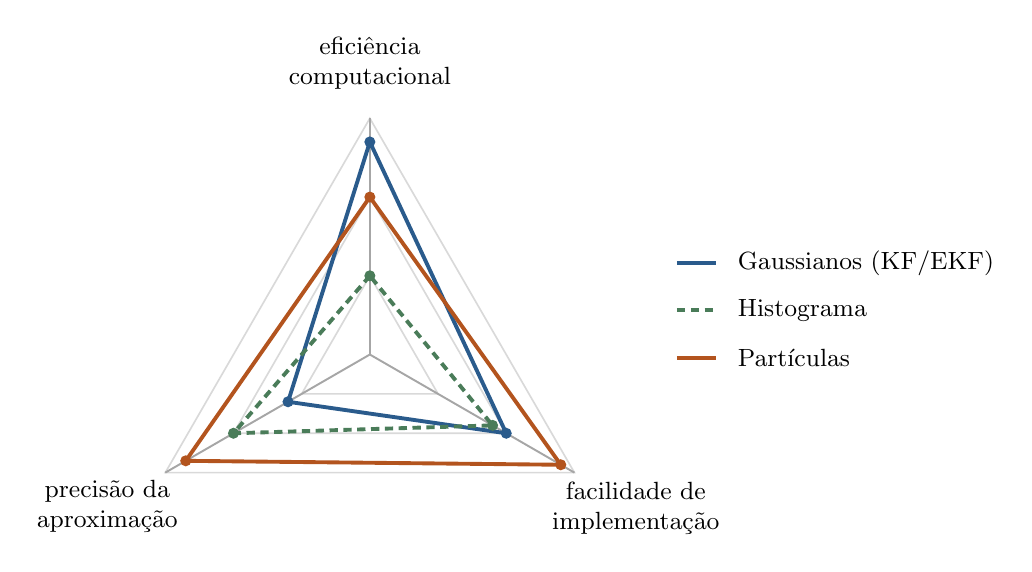
\begin{tikzpicture}[x=1cm,y=1cm]

  \def\R{3}   % raio da escala (valor máx = 3)

  % ----- grade -----
  \foreach \k in {1,2,3}
    \draw[black!15, line width=0.6pt] (90:\k) -- (210:\k) -- (330:\k) -- cycle;
  \foreach \a in {90,210,330}
    \draw[black!35, line width=0.7pt] (0,0) -- (\a:\R);

  % ----- rótulos dos eixos -----
  \node[align=center, font=\small] at (90:\R+0.7)  {eficiência\\computacional};
  \node[align=center, font=\small] at (210:\R+0.85) {precisão da\\aproximação};
  \node[align=center, font=\small] at (330:\R+0.9)  {facilidade de\\implementação};

  % ----- macro: \radar{cor}{estilo}{efic}{prec}{impl} (só contorno) -----
  \newcommand{\radar}[5]{%
    \draw[#1, line width=1.4pt, #2] (90:#3) -- (210:#4) -- (330:#5) -- cycle;
    \fill[#1] (90:#3) circle (2pt);
    \fill[#1] (210:#4) circle (2pt);
    \fill[#1] (330:#5) circle (2pt);
  }

  \radar{dblue}{solid}{2.7}{1.2}{2.0}          % Gaussianos (KF/EKF)
  \radar{dgreen}{densely dashed}{1.0}{2.0}{1.8} % Histograma
  \radar{dorange}{solid}{2.0}{2.7}{2.8}         % Partículas

  % ----- legenda -----
  \begin{scope}[shift={(3.9,1.0)}, font=\small]
    \draw[dblue,  line width=1.4pt] (0,0.16) -- (0.5,0.16);
    \node[anchor=west] at (0.65,0.16) {Gaussianos (KF/EKF)};
    \draw[dgreen, line width=1.4pt, densely dashed] (0,-0.44) -- (0.5,-0.44);
    \node[anchor=west] at (0.65,-0.44) {Histograma};
    \draw[dorange, line width=1.4pt] (0,-1.04) -- (0.5,-1.04);
    \node[anchor=west] at (0.65,-1.04) {Partículas};
  \end{scope}

\end{tikzpicture}
\end{document}
